% !TEX root = ../main.tex
\begin{figure}[t]
  \centering
  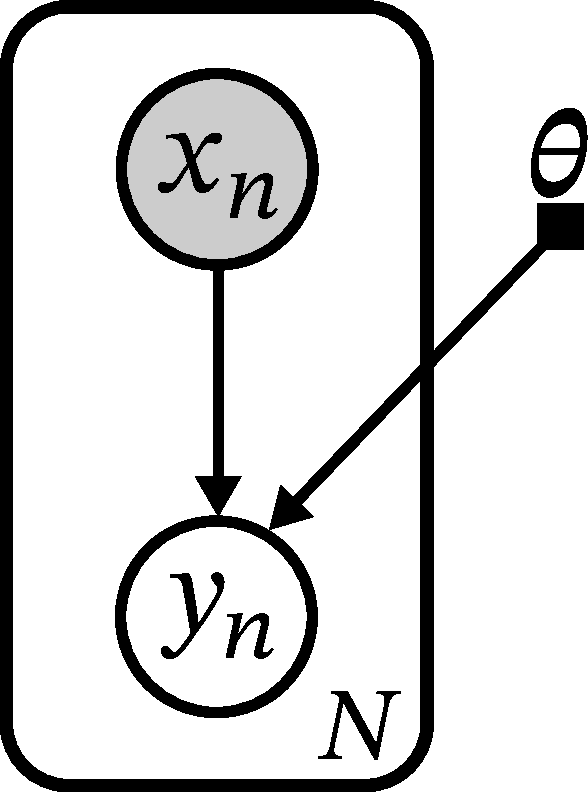
\includegraphics[height=0.2\paperheight]{fig/graphical-model-regression.pdf}
  \caption[Graphical model for logistic regression]{
  \textbf{Binary classification is a probabilistic modeling technique used in recommender systems.} Observed random variables are denoted by shaded nodes, and directed edges in the graph indicated conditional dependence on a node's parents. There are $N$ independent, identically distributed observations $(y_n, x_n)$; the rectangular plate denotes repetition of nodes and edges. The model predicts a binary response $y_n$ using parameters $\mbtheta$ and covariates $x_n$.}
  \label{fig:graphical-model-regression}
\end{figure}